\documentclass[a4paper,10pt]{beamer}
\usepackage{subcaption}
\usepackage{tikz}
\usetikzlibrary{positioning, shapes.geometric, calc, arrows.meta}
% \setbeameroption{show notes on second screen=right}

% Theme Choice
\usetheme{metropolis}
\usecolortheme{default}

% Title page
\title{Efficient Global Content Recovery for Multi-View Data}
\author{Ryan Jackson, David Zhao, Dowoo Kim}

\begin{document}
\metroset{block=fill} % Fill the block with the specified colors

\maketitle

\begin{frame}{Multi-view Data with Partial Observability}
  \begin{columns}[c]
    % Left Column: Text
    \begin{column}{0.45\textwidth}
      \textbf{Latent Factor Decomposition:}
      \vspace{-1.0em}
      \begin{itemize}
        \item<1-> \textbf{Observation ($\mathbf{x}_k$):} Data generated from content and style.
        \item<1-> \textbf{Style ($\mathbf{s}_k$):} View-specific factors (e.g., lighting).
        \item<1-> \textbf{Content ($\mathbf{c}$):} Shared invariant factors (e.g., identity).
      \end{itemize}
      \vspace{0.5em}
      \uncover<2->{
        \textit{Goal:} Identify $\mathbf{c}$ despite only observing partial subsets of the environment.
      }
    \end{column}
    % Right Column: Figure
    \begin{column}{0.5\textwidth}
      \begin{figure}
        \centering
        
\includegraphics[width=\textwidth]{figures/yao_multiview.png}
        \caption{Multi-view Data Setup. Source: Yao et al. (2024) \cite{yao2024multiviewcausalrepresentationlearning}.}
      \end{figure}
    \end{column}
  \end{columns}

\end{frame}

\begin{frame}{Example: Multimodal3DIdent}
  \begin{figure}[H]
    \centering
    \begin{subfigure}{0.45\textwidth}
      \includegraphics[width=\textwidth]{figures/multi_causal.png}
      \caption{Causal3DIdent: causal graph illustrating the data generation process \cite{julius_von_kugelgen_2021_4784282}.}
    \end{subfigure}
    \hfill
    \begin{subfigure}{0.45\textwidth}
      
\includegraphics[width=\textwidth]{figures/multi_example.png}
      \caption{Multimodal3DIdent: Examples of image-caption pairs from the dataset. Each view captures different subsets of latent factors \cite{daunhawer2023identifiabilityresultsmultimodalcontrastive}.}
    \end{subfigure}
    \caption{Example of multi-view data with partial observability.}
  \end{figure}
\end{frame}

\begin{frame}{The Challenge of Identifiability}
  \begin{columns}[t]
    % Left Column: Text
    \begin{column}{0.5\textwidth}
      \textbf{The Ideal: Full Identifiability}
      \begin{itemize}
        \item Recover \textit{every} latent factor individually ($c_1, c_2, \dots$).
        \item Mapping $\hat{\mathbf{c}}$ to $\mathbf{c}$ must be trivial (permutation/scaling).
      \end{itemize}

      \vspace{1em}
      \uncover<2->{
        \textbf{The Reality:}
        \begin{itemize}
          \item Requires latent variables to be independent and restrictive assumptions on the mixing functions.
          \item Unrealistic for real-world data.
        \end{itemize}
      }
    \end{column}
    % Right Column: Figure
    \begin{column}{0.5\textwidth}
      \begin{figure}
        \centering
        
\includegraphics[width=\textwidth]{figures/yao_multiview.png}
      \end{figure}
    \end{column}
  \end{columns}
\end{frame}

\begin{frame}{Relaxation: Block-Identifiability}
  \begin{block}{Definition}
    The true content $\mathbf{c}$ is \textbf{block-identified} \cite{julius_von_kugelgen_2021_4784282} by an encoder $g(\mathbf{x})$ if there exists a smooth invertible mapping $h$ such that:
    \[ \hat{\mathbf{c}} = g(\mathbf{x}) = h(\mathbf{c}) \]
  \end{block}

  \begin{columns}[t]
    \begin{column}{0.5\textwidth}
      \uncover<2->{
        \textbf{Key Properties}
        \begin{itemize}
          \item \textbf{Invariance:} $\hat{\mathbf{c}}$ captures the shared structure across views.
          \item \textbf{Isolation:} $\hat{\mathbf{c}}$ is independent of view-specific style $\mathbf{s}_k$.
        \end{itemize}
      }
    \end{column}
    \begin{column}{0.45\textwidth}
      \uncover<3->{
        \textbf{Why ``Block"?}
        \begin{itemize}
          \item We recover the joint information as a ``block" but it may be entangled.
          \item Sufficient for downstream causal tasks and prediction.
        \end{itemize}
      }
    \end{column}
  \end{columns}
\end{frame}

\begin{frame}{Contrastive Learning}
  \textbf{Contrastive Learning:} Maximize agreement between representations of different views of the same content while minimizing agreement between different contents.
  \begin{figure}
    \centering
    \includegraphics[width=0.8\textwidth]{figures/contrastive_learning.png}
    \caption{Contrastive learning example. Pictures of dogs (and cats) should be close in representation space, but dogs and cats should be far apart.}
  \end{figure}
\end{frame}

\begin{frame}{Block-Identification via Contrastive Learning}
  Yao et al. (2024) \cite{yao2024multiviewcausalrepresentationlearning} show that, under certain assumptions, contrastive learning can achieve block-identifiability of the content $\mathbf{c}$ in multi-view data by minimizing the contrastive loss:
  \begin{align*}
    \mathcal{L} = \underbrace{\sum_{k < k' \in V} \mathbb{E} \left[ \|g_k(\mathbf{x}_k) - g_{k'}(\mathbf{x}_{k'})\|_2 \right]}_{\text{Content Alignment}} - \underbrace{\sum_{k \in V} H(g_k(\mathbf{x}_k))}_{\text{Entropy regularization}},
  \end{align*}
  where \textcolor<2>{red}{$g_k : \mathcal{X}_k \to \mathbb{R}^{|\mathbf{c}|}$} is the encoder for view $k$, and $H(\cdot)$ denotes the differential entropy.
  \vfill
  \uncover<2->{
    \begin{alertblock}{The Known Content Dimension Constraint}
      The dimensionality of the encoder output \textbf{must exactly match} the true content dimension: $\dim(\hat{\mathbf{c}}) = \dim(\mathbf{c})$.
    \end{alertblock}
  }
\end{frame}

\begin{frame}{The Known Content Dimension Constraint}
  This is a very strong requirement that is often violated in practice:
  \begin{itemize}
    \item \textbf{Underestimation:} If $\dim(\hat{\mathbf{c}}) < \dim(\mathbf{c})$, we lose information and cannot recover the full content.
    \item \textbf{Overestimation:} If $\dim(\hat{\mathbf{c}}) > \dim(\mathbf{c})$, the encoder may capture spurious style information, leading to entangled representations and loss of block-identifiability.
  \end{itemize}
\end{frame}

\begin{frame}{A masking approach}
  Yao et al. (2024) \cite{yao2024multiviewcausalrepresentationlearning} show that for view-specific encoders $R = \{r_k\}$, content selectors $\Phi = \{\phi_V^k\}$, and projections $T = \{t_k\}$ solving:
  \begin{equation*}
    \min \text{Reg}(\Phi) := \sum_{V \in \mathcal{V}} \sum_{k \in V} \| \phi_V^{k} \|_0 \quad \text{subject to:} \quad R, \Phi, T \in \arg\min \mathcal{L}(R, \Phi, T)
  \end{equation*}
  where $\text{Reg}(\Phi)$ is an $L_0$ sparsity penalty on the selectors, and the base loss is:
  \begin{align*}
    \mathcal{L}(R, \Phi, T) &= \sum_{V \in \mathcal{V}} \sum_{k < k' \in V} \mathbb{E} \left[ \|\phi_V^k \oslash r_k(\mathbf{x}_k) - \phi_V^{k'} \oslash r_{k'}(\mathbf{x}_{k'})\|_2 \right] \\
    &- \sum_{k \in V} H(t_k \circ r_k(\mathbf{x}_k))
  \end{align*}
  Then for any $V \in \mathcal{V}$ and $k \in V$, the masked representation $\phi_V^k \oslash r_k$ block-identifies $\mathbf{z}_{C_V}$.
  \vfill
  \uncover<2->{
    \begin{alertblock}{Known View-Specific Latent Dimension Constraints}
      The view-specific encoders are assumed to map to the exact dimension matching the true dimension of the subset of latents generating the view.
    \end{alertblock}
  }
\end{frame}

\begin{frame}{Literature Overview: Handling Unknown $|c|$}
  \begin{description}
    \item<1->[\textbf{1. Heuristic Search}] \textit{(Traditional)} \\
      Iterative training with different $|\hat{\mathbf{c}}|$ values.
      \begin{itemize}
        \item \textbf{Drawback:} Extremely computationally expensive and unsatisfactory.
      \end{itemize}
    \item<2->[\textbf{2. Dimensionality Reduction}] \textit{(Post-hoc)} \\
      Train encoders and apply PCA or ICA on the representations.
      \begin{itemize}
        \item \textbf{Drawback:} Standard DR techniques don't respect the \textit{causal} block structure; style often stays mixed with content.
      \end{itemize}
    \item<3->[\textbf{3. Sparsity-Inducing Penalties}] \textit{(Modern)} \\
      Using $\ell_0$ regularization to prune dimensions during training.
      \begin{itemize}
        \item \textbf{Drawback:} Non-differentiable and computationally expensive.
      \end{itemize}
  \end{description}
  \note{
    \begin{itemize}
      \item Treat as hyperparameter and searching over it. Very computationally expensive since need to retrain for each candidate output dimension. Use elbow plots, but still unreliable.
      \item Post-hoc dimensionality reduction: style and content are often entangled in messy ways. PCA/ICA don't know how to separate them.
      \item Sparsity-inducing penalties: combinatorial nightmare.
    \end{itemize}
  }
\end{frame}

\begin{frame}{Our Proposed Method}
  We introduce a \textit{learnable shared global gate} $\mathbf{\phi} \in [0,1]^{\mathrm{dim}(\hat{c})}$ applied to the output of all view encoders, by means of a hard concrete distribution \cite{louizos2018learningsparseneuralnetworks}:
  \begin{columns}[c]
    \begin{column}{0.5\textwidth}
      \begin{itemize}
        \item \textbf{Stochastic Binary Mask}
        \item \textbf{Continuous relaxation of $\ell_0$}
        \item \textbf{Differentiable end-to-end training}
      \end{itemize}
    \end{column}
    \begin{column}{0.5\textwidth}
      \begin{figure}
        \centering
        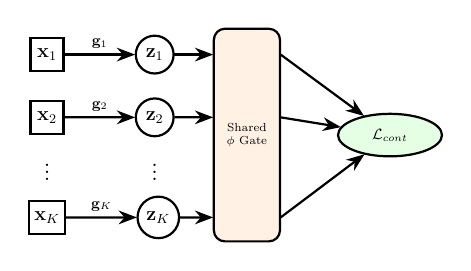
\begin{tikzpicture}[
            >=Stealth,
            scale=0.6,
            transform shape,
            node distance=0.5cm and 1.5cm, % Increased horizontal distance for label clarity
            % Styles
            input/.style={rectangle, draw, thick, minimum size=0.7cm, font=\large},
            rep/.style={circle, draw, thick, minimum size=0.8cm, font=\large},
            gate/.style={
              rectangle, draw, fill=orange!10,
              minimum height=4.5cm, minimum width=1.4cm,
              align=center, rounded corners, font=\scriptsize, thick
            },
            loss/.style={
              ellipse, draw, fill=green!10,
              minimum height=0.9cm, minimum width=2.2cm,
              align=center, font=\small, thick
            }
          ]
          % 1. Inputs (x) in Squares
          \node[input] (x1) {$\mathbf{x}_1$};
          \node[input, below=0.6cm of x1] (x2) {$\mathbf{x}_2$};
          \node[below=0.3cm of x2, font=\Large] (xdots) {$\vdots$};
          \node[input, below=0.3cm of xdots] (xK) {$\mathbf{x}_K$};
          % 2. Representations (z) in Circles
          \node[rep, right=of x1] (z1) {$\mathbf{z}_1$};
          \node[rep, right=of x2] (z2) {$\mathbf{z}_2$};
          \node[font=\Large] (zdots) at (xdots -| z1) {$\vdots$};
          \node[rep, right=of xK] (zK) {$\mathbf{z}_K$};
          % 3. Shared Gate (phi)
          \path (z1) -- (zK) coordinate[midway] (midZ);
          \node[gate, right=1.2cm of midZ] (phi) {Shared\\$\mathbf{\phi}$ Gate};
          % 4. Contrastive Loss
          \node[loss, right=1.2cm of phi] (loss) {$\mathcal{L}_{cont}$};
          % --- Connections ---
          \foreach \i in {1,2,K} {
            % Arrow from x to z with g_i on top
            \draw[->, thick] (x\i) -- node[above, font=\small] {$\mathbf{g}_{\i}$} (z\i);
            % Connections to the gate and loss
            \draw[->, thick] (z\i) -- (phi.west |- z\i);
            \draw[->, thick] (phi.east |- z\i) -- (loss);
          }
        \end{tikzpicture}
        \caption{Global Gating Architecture}
      \end{figure}
    \end{column}
  \end{columns}
  \note{
    \begin{itemize}
      \item Original paper from Louizos et al. (2018) \cite{louizos2018learningsparseneuralnetworks} proposed the hard concrete distribution for learning sparse neural networks. We adapt this idea to our multi-view setting by introducing a shared global gate that applies to all view encoders.
      \item Prune dimensions during training to encourage the model to learn a sparse representation that captures only the shared content dimensions.
      \item Explain figure.
      \item Stochastic binary mask: learns the probability of turning on/off each dimension.
      \item Continuous relaxation: allows for gradient-based optimization.
      \item End-to-end training: no need for a separate pruning phase (e.g. post-hoc DR)
    \end{itemize}
  }
\end{frame}

\begin{frame}{Numerical Experiment: Independent Factors}
  \begin{columns}[c]
    \begin{column}{0.4\textwidth}
      \textbf{Setup Details:}
      \begin{itemize}
        \item 8 views, 10 total latents.
        \item \textbf{Gaussian latents:} $\mathbf{z} \sim \mathcal{N}(\mathbf{0}, \mathbf{I})$.
        \item $\mathbf{z_1}, \mathbf{z}_2$ are shared content.
        \item $\mathbf{z}_3, \dots, \mathbf{z}_{10}$ are view-specific style.
        \item Overestimate content dimension: $\dim(\hat{\mathbf{c}}) = 6$.
      \end{itemize}
    \end{column}
    \begin{column}{0.6\textwidth}
      \centering
      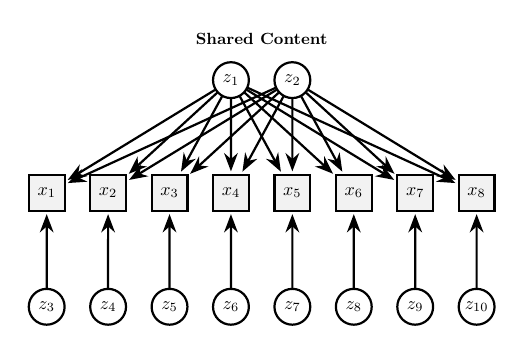
\begin{tikzpicture}[scale=0.65, transform shape,
          node distance=1.5cm and 0.3cm,
          latent/.style={circle, draw, thick, inner sep=1pt, minimum size=7mm},
          obs/.style={rectangle, draw, thick, fill=gray!10, inner sep=2pt, minimum size=7mm},
          arrow/.style={-Stealth, thick, shorten >=1pt},
          label/.style={font=\small\bfseries}
        ]
        \foreach \i in {1,...,8} {
          \node[obs] (x\i) at ({(\i-4.5)*1.2cm}, 0) {$x_{\i}$};
        }
        \node[latent] (c1) at (-0.6cm, 2.2cm) {$z_1$};
        \node[latent] (c2) at (0.6cm, 2.2cm) {$z_2$};
        \node[above=0.2cm of c1, xshift=0.6cm, label] {Shared Content};
        \foreach \i [evaluate=\i as \latentidx using int(\i+2)] in {1,...,8} {
          \node[latent, below=of x\i] (s\i) {$z_{\latentidx}$};
        }
        \foreach \i in {1,...,8} {
          \draw[arrow] (c1) to (x\i);
          \draw[arrow] (c2) to (x\i);
          \draw[arrow] (s\i) to (x\i);
        }
      \end{tikzpicture}
    \end{column}
  \end{columns}
  \note{
    \begin{itemize}
      \item We generate synthetic data with 8 views and 10 latent factors. Standard Gaussian independent latents.
      \item Assume we don't know the true content dimension, so we set the encoder output dimension to 6, and see if the model can learn to gate out the 4 spurious style dimensions and recover the 2 shared content dimensions.
    \end{itemize}
  }
\end{frame}

\begin{frame}{Numerical Results - Independent Latent Factors}
  \begin{figure}[H]
    \centering
    \begin{subfigure}{0.45\textwidth}
      
\includegraphics[width=\textwidth]{figures/numerical_indep_gate_history.png}
      \caption{Gate convergence history}
    \end{subfigure}
    \hfill
    \begin{subfigure}{0.45\textwidth}
      
\includegraphics[width=\textwidth]{figures/numerical_indep_r2.png}
      \caption{$R^2$ performance per latent factor.}
    \end{subfigure}
    \caption{Numerical Experiment Results (\textbf{independent} latent factors).}
  \end{figure}
  \note{
    \begin{itemize}
      \item Gate convergence history: gate values for the 6 encoder dimensions over training. 2 dimensions converge to 1, rest converge to 0.
      \item Representations live in 2-dim subspace of 6-dim output space. Sparse representation.
      \item How well does it perform? Despite sparse representation, after training a linear reg model to predict each latent factor from the gated representation, we achieve perfect $R^2$ performance on the 2 content dimensions, and near-zero performance on the 4 style dimensions.
      \item We use $R^2$ because it tells us how well we can predict the true latent factor from the learned representation, which is a direct measure of block-identifiability.
    \end{itemize}
  }
\end{frame}

\begin{frame}{Numerical Results - Dependent Latent Factors}
  \begin{figure}[H]
    \centering
    \begin{subfigure}{0.45\textwidth}
      
\includegraphics[width=\textwidth]{figures/numerical_dep_gate_history.png}
      \caption{Gate convergence history}
    \end{subfigure}
    \hfill
    \begin{subfigure}{0.45\textwidth}
      
\includegraphics[width=\textwidth]{figures/numerical_dep_r2.png}
      \caption{$R^2$ performance per latent factor.}
    \end{subfigure}
    \caption{Numerical Experiment Results (\textbf{dependent} latent factors).}
  \end{figure}
  \note{
    \begin{itemize}
      \item This time, we allow arbitrary dependencies between the latent factors, which is more realistic for real-world data.
    \end{itemize}
  }
\end{frame}

\begin{frame}{Multimodal3DIdent Results}
  \begin{figure}[H]
    \centering
    \begin{subfigure}{0.45\textwidth}
      
\includegraphics[width=\textwidth]{figures/multimodal_gate_history.png}
      \caption{Gate convergence history}
    \end{subfigure}
    \hfill
    \begin{subfigure}{0.45\textwidth}
      
\includegraphics[width=\textwidth]{figures/multimodal_r2.png}
      \caption{Prediction performance per latent factor.}
    \end{subfigure}
    \caption{Multimodal Experiments on Multimodal3DIdent Dataset.}
  \end{figure}
  \note{
    \begin{itemize}
      \item Multimodal3DIdent: image-caption pairs. Only 3 shared content dimensions (object color, object x pos, object y pos).
      \item Overestimate to 32 dimensions. Model recovers exactly 3 dimensions, with comparable $R^2$ performance to Daunhawer (creator of the dataset who assumed known content dimension).
    \end{itemize}
  }
\end{frame}

\begin{frame}{Discussion}
  \textbf{Key Takeaways:}
  \begin{itemize}
    \item Our global gating method successfully identifies the correct number of content dimensions in both synthetic and real multimodal datasets.
    \item The method is robust to overestimation of the content dimension, consistently recovering the shared content structure without significant entanglement with style.
  \end{itemize}
  \note{
    \begin{itemize}
      \item Despite having no foreknowledge of the true content dimension, our method learns to gate out the spurious dimensions and recover the correct number of content dimensions.
      \item Very robust: Even in cases where latent factors are dependent, and in real-world multimodal data, our method still successfully recovers the shared content structure.
    \end{itemize}
  }
\end{frame}

\begin{frame}{Limitations \& Future Work}
  \textbf{Lack of Formal Proofs:} While empirical results are strong, the theoretical guarantees for block-identifiability under the \textit{relaxed overestimation} setting are yet to be established.
  \vfill
  \uncover<2->{
    \textbf{Future Research Directions}
    \begin{itemize}
      \item \textbf{Theoretical Conditions:} Establish formal requirements for block-identifiability when content dimensions are overestimated.
      \item \textbf{Sensitivity Analysis:} Investigate how the \textit{degree} of overestimation affects training convergence/cost.
    \end{itemize}
  }
  \note{
    \begin{itemize}
      \item Exciting empirical results, but no theoretical proofs for block-identifiability under overestimation.
    \end{itemize}
  }
\end{frame}

\begin{frame}{Conclusion}
  \textbf{Summary:}
  \begin{itemize}
    \item We introduced a method for block-identifiable content recovery in multi-view data with partial observability, where the content dimension is unknown and potentially overestimated.
    \item Our approach leverages a shared global gate to learn a sparse representation during training.
    \item Empirical results on synthetic and real datasets demonstrate that the true number of content dimensions are matched, with comparable prediction performances.
  \end{itemize}
  \note{
    \begin{itemize}
      \item Proposed shared gating method for block-identifiable content recovery when content dimension is unknown and overestimated.
      \item Method tries to learn a sparse representation that captures only the shared content dimensions.
      \item Empirical results are very strong and comparable to prior work that assumed known content dimension.
    \end{itemize}
  }
\end{frame}

\begin{frame}{References}
  \footnotesize
  \bibliographystyle{unsrt}
  \bibliography{ref.bib}
\end{frame}
\end{document}
